\mychapter{1}{Lesson 1} %180926

\section{Secret communication}

The typical setting for the problem of secret communication is depicted in figure \ref{fig:secrecy}. The parties Alice and Bob want to share data in a private fashion, and thus prevent a third party Eve form learning the shared data, in a word, \emph{eavesdropping}. The objects used here are:
\begin{itemize}
    \item The data to be shared, or \emph{message} $m$;
    \item Some secret information, shared between Alice and Bob, that is used to \emph{encrypt} the message: the \emph{encryption key} or just \emph{key} $k$;
    \item The result of encrypting a message $m$ using the key $k$: the ciphertext $c$.
\end{itemize}

\begin{figure}[ht]
    \centering
    \begin{tikzpicture}
        \draw
            (0, 0) node (a) [box, fill = white] {Alice} 
            (5, 0) node (b) [box, fill = white] {Bob}
            (2.5, -1) node (e) [box, fill = white] {Eve}
        ;

        \draw[-Stealth] (a) -- node [midway, above] {$c$} (b);
        \draw[-Stealth] (0, -1) node [below] {$k$} -- (a);
        \draw[-Stealth] (5, -1) node [below] {$k$} -- (b);
        \draw[-Stealth] (-1, 0) node [left] {$m$} -- (a);
        \draw[-Stealth] (b) -- (6, 0) node [right] {$m$};
        \draw[-Stealth] (2, -0.1) -- (3, -0.1)
            (2.5, -0.1) -- (e);

    \end{tikzpicture}

    \caption{A depiction of the problem of secret communication}
    \label{fig:secrecy}
\end{figure}

To complete the picture, the two parties Alice and Bob use a \emph{cryptographic secrecy scheme}, or \emph{encryption scheme} to convert the message in an encrypted form, and vice versa. It has the form $\Xi = (\Enc, \Dec)$, where:
\begin{itemize}
    \item $\Enc \in \K \times \M \to \C$ is the function that, given a message $m$ in $\M$ and a key $k$ in $\K$ performs the encryption, and thus generates the corresponding ciphertext $c$ in $\C$;
    \item $\Dec \in \K \times \C \to \M$ restores a message starting from the ciphertext and the key originally used in the encryption.
\end{itemize}

Thus, for a secrecy scheme to work as intended, the following statement must hold:
\[
    \forall m \in \M \, \forall k \in \K \quad \Dec(k, \Enc(k, m)) = m
\]

\begin{definition}[Shannon's perfect secrecy]
    Let $M$ be a generic random variable over $\M$, and $K$ a uniform random variable over $\K$. Then, the cryptosystem $\Xi: (\Enc, \Dec)$ is deemed \emph{perfectly secret} iff the ciphertext $C = \Enc(K, M)$ obtained by encrypting the random message $M$ using the uniformly random key $K$ is effectively useless in retrieving any information about the original message:
    \[
        \forall M \sim \mathcal{R}and(\M) \, \forall C \simeq \Enc(K, M) \quad \Pr[M = m] = \Pr[M = m \knowing C = c]
    \]
\end{definition}

The perfect secrecy definition can be rephrased in different ways, bringing more details to light:
    
\begin{proposition}
    The following statements are equivalent:
    \begin{enumerate}
        \item \label{def:ps1} $\Pr[M = m] = \Pr[M = m \knowing C = c]$
        \item \label{def:ps2} $M \indep C$
        \item \label{def:ps3} $\forall m_1, m_2 \in \M \, \forall c \in \C \quad \Pr[\Enc(K, m_1) = c] = \Pr[\Enc(K, m_2) = c]$
    \end{enumerate}
\end{proposition}

\begin{proof}
    The proof is structured as a cyclic implication between the three definitions:
    
    \begin{itemize}
        \item $(\ref{def:ps1}) \implies (\ref{def:ps2})$: Start from one side of the independency definition, and work through the other:
        \begin{align*}
             & \Pr[C = c \wedge M = m]              & \\
            =& \Pr[C = c] \Pr[M = m \knowing C = c] & \text{(Conditional prob.)} \\
            =& \Pr[C = c] \Pr[M = m]                & \text{(Using 1.)} \\
        \end{align*}
        This proves that $M$ and $C$ are independent distributions.
        
        \item $(\ref{def:ps2}) \implies (\ref{def:ps3})$: Let $M$ be a generic random variable over $\M$. Then:
        \begin{align*}
             & \Pr[\Enc(K, m_1) = c]                & \\
            =& \Pr[\Enc(K, M) = c \knowing M = m_1] & \text{(Introducing $M$)} \\
            =& \Pr[C = c \knowing M = m_1]          & \text{($C$ definition)} \\
            =& \Pr[C = c]                           & \text{(Using 2.)} \\
            =& \Pr[\Enc(K, m_2) = c]                & \text{(Same steps reversed, where $m_1 \mapsto m_2$)}\\
        \end{align*}

        \item $(\ref{def:ps3}) \implies (\ref{def:ps1})$:
        \begin{align*}
             & \Pr[C = c]                                                   & \\
            =& \sum_{m \in \M}\Pr[C = c \wedge M = m]                       & \text{(Total prob.)} \\
            =& \sum_{m \in \M}\Pr[\Enc(K, M) = c \wedge M = m]              & \text{($C$ definition)} \\
            =& \sum_{m \in \M}\Pr[\Enc(K, M) = c \knowing M = m] \Pr[M = m] & \text{(Conditional prob.)} \\
            =& \sum_{m \in \M}\Pr[\Enc(K, m) = c] \Pr[M = m]                & \text{(Condition collapse)} \\
            =& \Pr[\Enc(K, \overline{m}) = c] \sum_{m \in \M} \Pr[M = m]    & \text{(Using 3.)} \\
            =& \Pr[\Enc(K, \overline{m}) = c]                               & \text{(Total prob.)} \\
            =& \Pr[\Enc(K, M) = c \knowing M = \overline{m}]                & \text{(Condition expansion)} \\
            =& \Pr[C = c \knowing M = \overline{m}]                         & \text{($C$ definition)} \\
        \end{align*}

        Knowing this, and applying Bayes' theorem, we get back to the first definition:
        \begin{align*}
                    & \Pr[C = c] = \Pr[C = c \knowing M = m]                                        & \\
            \implies& \Pr[C = c] = \Pr[M = m \knowing C = c] \cdot \frac{\Pr[C = c]}{\Pr[M = m]}    & \text{(Bayes' theorem)} \\
            \implies& \Pr[M = m] = \Pr[M = m \knowing C = c]                                        & \\
        \end{align*}
    \end{itemize}
\end{proof}

A remark on definition \ref{def:ps3} has to be done here:
\begin{align*}
        & \Pr[\Enc(K, m) = c] \\
       =& \Pr[\Enc(K, M) = c \knowing M = m] \\
    \neq& \Pr[\Enc(K, M) = c]
\end{align*}

which is exactly the difference between \emph{choosing} a specific message $m$, and picking it at random, as $M$ suggests.

\subsection{One-time Pad}

The One-time Pad, or \otp{} in short, is a fairly simple scheme that leverages the involutory property of the \textsc{xor} operation. Let all the spaces $\K$, $\M$ and $\C$ be binary strings of some length $\binary^l$, and define the following cryptographic scheme:
\begin{itemize}
    \item $\Enc(k, m) = k \oplus m = c$
    \item $\Dec(k, c) = k \oplus c = m$
    \item Correctness: $\Dec(k, \Enc(k, m)) = \Dec(k, k \oplus m) = k \oplus k \oplus m = m$.
\end{itemize}

\begin{theorem}
    \otp{} is perfectly secret.
\end{theorem}
\begin{proof}
    The proof is essentially a retelling of the steps used for proving that the second definition of perfect secrecy implies the third one. Let $K \sim \unifdist(\K)$. Then, $\forall m_1, m_2, c \in \binary^l$:
    \begin{align*}
        & \Pr[\Enc(K, m_1) = c]     & \\
        =& \Pr[K \oplus m_1 = c]    & \\
        =& \Pr[K = c \oplus m_1]    & \\
        =& \oneover{|\K|}           & \text{(K is uniform)} \\
        =& \Pr[\Enc(K, m_2) = c]    & \text{(Same steps reversed, where $m_1 \mapsto m_2$)} \\  
    \end{align*}
    This satisfies the third definition of perfect secrecy.
\end{proof}

%TODO OLD NOTE: Observation: k is truly random, but fixed, compare with Pi_\oplus's encryption routine: from a security standpoint, nothing changes! actually, \Pi_\oplus may be weaker brute-force wise than OTP!

By observing our recent proof, some insights (and problems) arise:
\begin{enumerate}
    \item The key and the message's lengths must always match ($|k| = |m|$);
    \item As the name suggests, keys are useful just for one encryption. Otherwise, given two encryptions with the same key, an attacker may exploit the \textsc{xor}'s idempotency to extract valuable information from both ciphertexts\footnote{This vulnerability of applying a function on a ciphertext, and expecting as a result the image of the original message by the same function, is called \emph{malleability}, and is explored further in the notes.}:
    \[
        c_1 = k \oplus m_1 \wedge c_2 = k \oplus m_2 \implies c_1 \oplus c_2 = m_1 \oplus m_2
    \]
    
\end{enumerate}

%\footnote{An encryption algorithm is "malleable" if it is possible to transform a ciphertext into another ciphertext which decrypts to a related plaintext. That is, given an encryption $c$ of a plaintext $m$, it is possible to generate another valid ciphertext $c'$, for a known $Enc$, $Dec$, without necessarily knowing or learning $m$.}

Combined with the fact that keys must be preemptively shared in a secure fashion, these problems make for a quite impractical cryptographic scheme. One can further this analysis and generalize it to all ``perfect'' schemes, giving a rather delusive conclusion:

\begin{figure}[h]
    \centering
    \def\firstcircle{(0,0) circle (1.5cm)}
    \def\secondcircle{(60:0) circle (0.9cm)}
    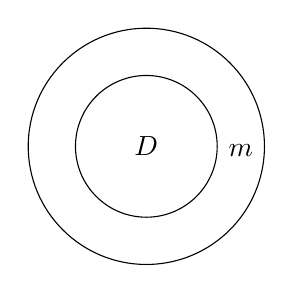
\begin{tikzpicture}
        \begin{scope}[shift={(3cm,-5cm)}]
            \draw \firstcircle node[label={[xshift=1.0cm, yshift=0.3cm]$\M$}] { };
            \draw \secondcircle node[label={[xshift=1.2cm, yshift=-0.5cm]$m$}] {$D$};
        \end{scope}
    \end{tikzpicture}
    \caption{Where the messages stand}
\end{figure}

\begin{theorem}
    For a secrecy scheme to be perfectly secret: $|\K| \geq |\M|$
\end{theorem}
\begin{proof}
    Perfection will be disproved by breaking definition \ref{def:ps1}. Let $M \sim \unifdist(\M)$, and take $c \in \C : \Pr[C = c] > 0$. Consider $D = \{\Dec(k, c) : k \in \K\}$ as the set of all images of the decryption routine with all keys in $\K$. The offending assumption is that $|\K| < |\M|$. Then, by how $D$ is defined:

    \[
        |D| \leq |\K| < |\M| \implies \exists m \in \M \setminus D
    \]

    Fix this message $m$, and remember that by $M$'s definition, $\Pr[M = m] = |\M|^{-1}$. Since $m \notin D$, there can be no key in $\K$ such that $\Dec(k, c) = m$. By observing that $C$ strictly distributes over $D$, where $m$ is not present, $\Pr[M = m \knowing C = c] = 0$. Putting everything together:
    \[
        0 = \Pr[M = m \knowing C = c] \neq \Pr[M = m] = |\M|^{-1}
    \]
    This clearly violates the first definition of perfect secrecy.
\end{proof}
